\section{LEP und der OPAL Detektor}
\subsection{LEP am CERN}
%LEP luftaufnahme
\begin{frame}
	\frametitle{Der LEP Speicherring}
	\begin{figure}
		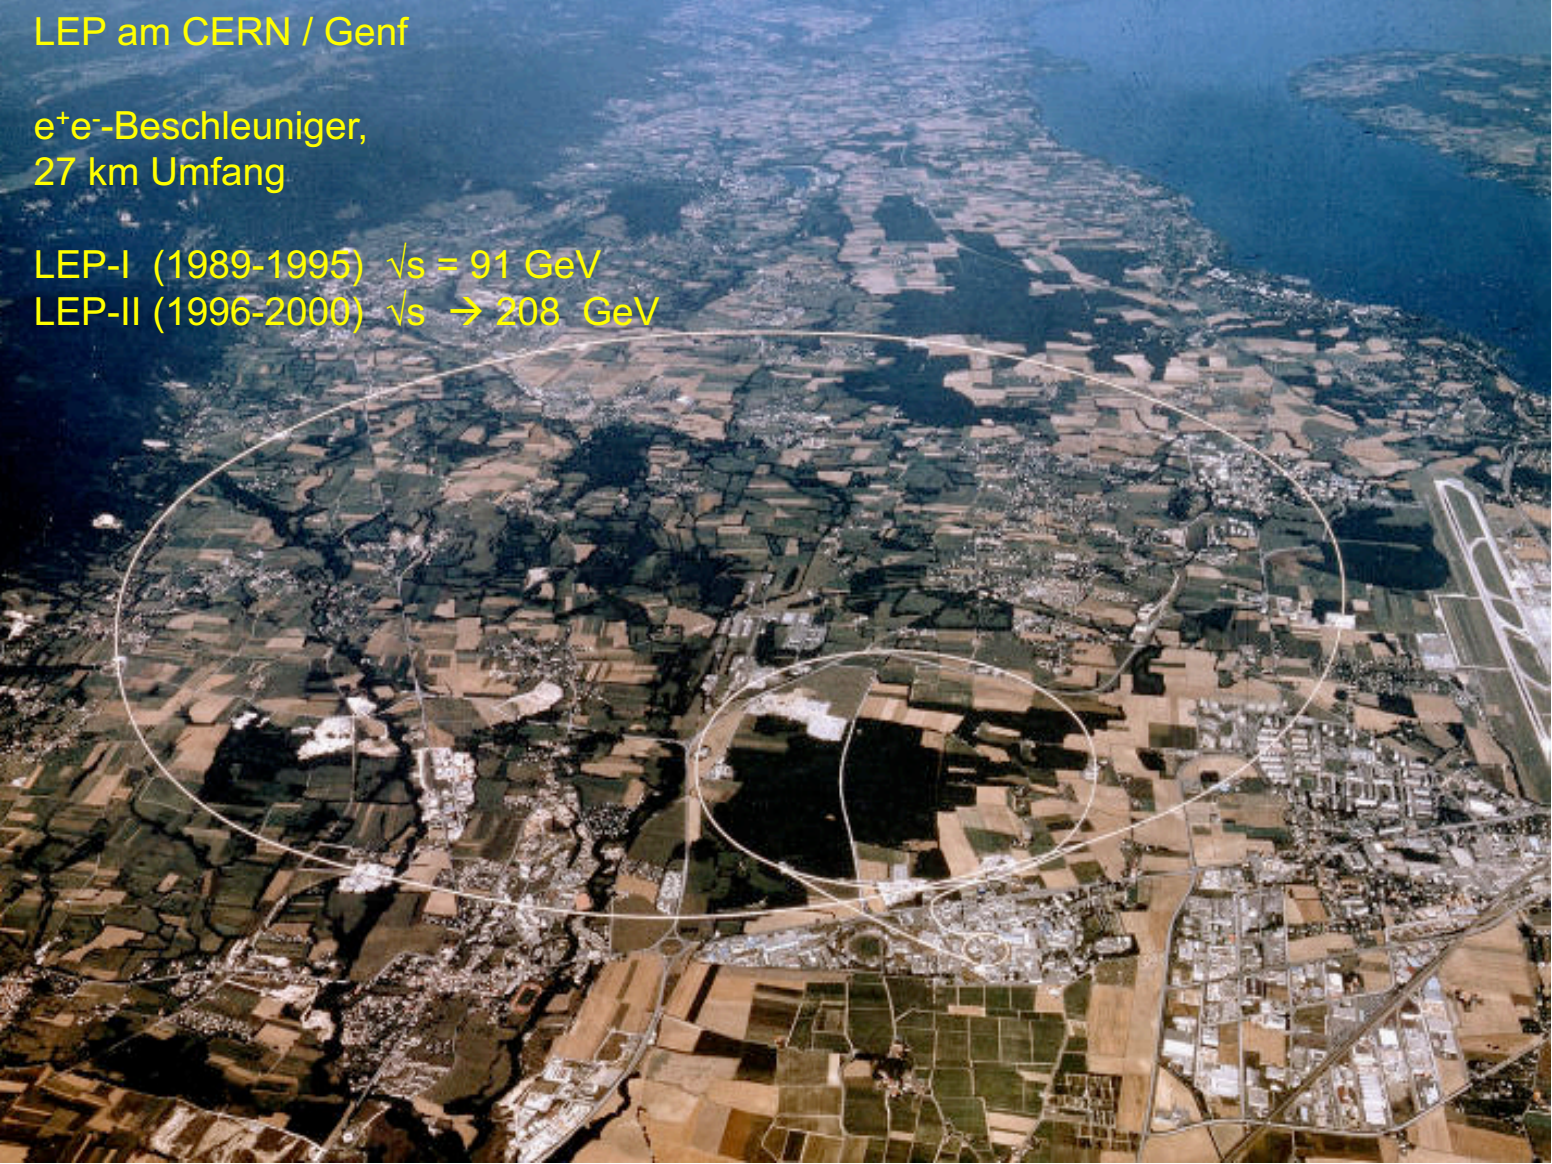
\includegraphics[width=1.0\linewidth]{graphics/LEPmap}
	\end{figure}
\end{frame}

\subsection{Der OPAL Detektor}
\begin{frame}
	\frametitle{Schematischer Aufbau}
	\begin{center}
	\begin{figure}
		\includegraphics[width=0.7\linewidth]{graphics/OPALaufbau}
	\end{figure}
	\end{center}
\end{frame}

\begin{frame}
	\frametitle{Driftkammer}
	\begin{center}
		\begin{figure}
			\includegraphics[width=0.75\linewidth]{graphics/slice_tracking_tr}
		\end{figure}
	\end{center}
\end{frame}

\begin{frame}
	\frametitle{Elektromagnetisches Kalorimeter}
	\begin{center}
		\begin{figure}
			\includegraphics[width=0.75\linewidth]{graphics/slice_calorimeter_tr}
		\end{figure}
	\end{center}
\end{frame}

\begin{frame}
	\frametitle{Myonenkammer}
	\begin{center}
		\begin{figure}
			\includegraphics[width=0.75\linewidth]{graphics/slice_muon_tr}
		\end{figure}
	\end{center}
\end{frame}


